% Triton kernel speedup bar chart
% Compile: pdflatex kernel_speedup.tex
% Inline:  % Triton kernel speedup bar chart
% Compile: pdflatex kernel_speedup.tex
% Inline:  % Triton kernel speedup bar chart
% Compile: pdflatex kernel_speedup.tex
% Inline:  % Triton kernel speedup bar chart
% Compile: pdflatex kernel_speedup.tex
% Inline:  \input{figures/kernel_speedup.tex}
%
% 数据来源:
%   profile_v2_h800.md   (forward-only)
%   profile_bwd_h800.md  (forward + backward)
% 测试硬件: NVIDIA H800 PCIe
% 测试形状: B=64, T=3072, d_model=448, d_ff=1216, h=7, V=256, bf16
%
% 设计要点:
%   - y 轴 log scale: 数据从 0.01x (linear_ce) 到 63.75x (ce_zloss) 跨 4 个数量级
%   - x 轴按 forward-only 加速比降序排列, 视觉趋势从高到低 + 反面案例垫底
%   - 柱顶数据标签竖排, 双工作负载分组对照
\documentclass[tikz,border=10pt]{standalone}
\usepackage{pgfplots}
\usepackage{amsmath}
\pgfplotsset{compat=1.18}

\begin{document}
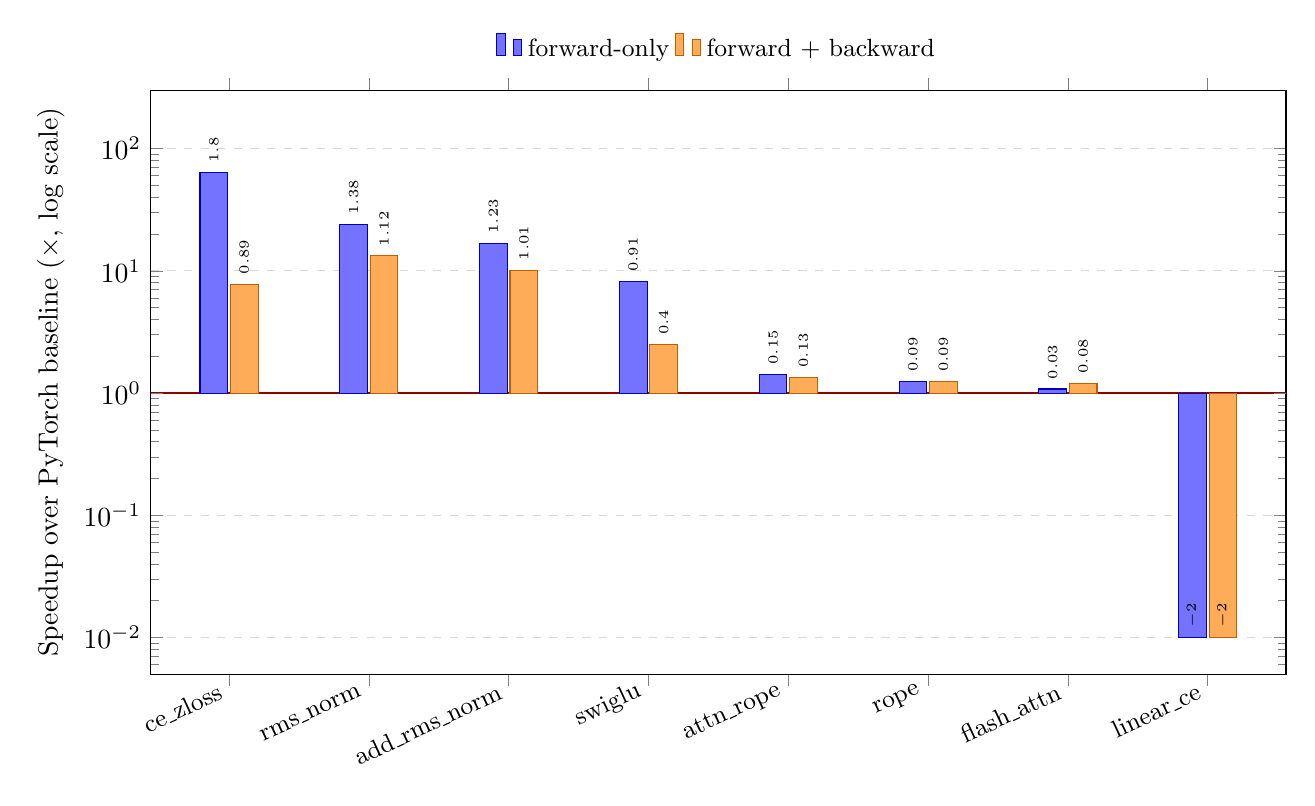
\begin{tikzpicture}
\begin{axis}[
    ybar=1pt,
    bar width=10pt,
    width=16cm,
    height=9cm,
    ymode=log,
    log basis y=10,
    ymin=0.005,
    ymax=300,
    ylabel={Speedup over PyTorch baseline ($\times$, log scale)},
    symbolic x coords={
        ce\_zloss,
        rms\_norm,
        add\_rms\_norm,
        swiglu,
        attn\_rope,
        rope,
        flash\_attn,
        linear\_ce
    },
    xtick=data,
    x tick label style={rotate=25, anchor=east, font=\small},
    enlarge x limits=0.08,
    legend style={
        at={(0.5,1.03)},
        anchor=south,
        legend columns=2,
        font=\small,
        draw=none
    },
    ymajorgrids=true,
    grid style={dashed, gray!30},
    extra y ticks={1},
    extra y tick labels={},
    extra y tick style={
        grid=major,
        grid style={solid, red!55!black, line width=0.6pt}
    },
    nodes near coords,
    every node near coord/.append style={
        font=\tiny,
        rotate=90,
        anchor=west,
        /pgf/number format/.cd, fixed, precision=2
    },
]

% forward-only speedup (蓝色) — 数据来自 profile_v2_h800.md
\addplot[fill=blue!55, draw=blue!70!black] coordinates {
    (ce\_zloss,       63.75)
    (rms\_norm,       24.00)
    (add\_rms\_norm,  16.82)
    (swiglu,           8.15)
    (attn\_rope,       1.42)
    (rope,             1.24)
    (flash\_attn,      1.08)
    (linear\_ce,       0.01)
};
\addlegendentry{forward-only}

% forward + backward speedup (橙色) — 数据来自 profile_bwd_h800.md
\addplot[fill=orange!65, draw=orange!75!black] coordinates {
    (ce\_zloss,        7.79)
    (rms\_norm,       13.26)
    (add\_rms\_norm,  10.13)
    (swiglu,           2.49)
    (attn\_rope,       1.34)
    (rope,             1.24)
    (flash\_attn,      1.20)
    (linear\_ce,       0.01)
};
\addlegendentry{forward + backward}

% baseline 1x 红色实线 (extra y tick + grid style 自动生成, 无需 \draw)

\end{axis}
\end{tikzpicture}
\end{document}

%
% 数据来源:
%   profile_v2_h800.md   (forward-only)
%   profile_bwd_h800.md  (forward + backward)
% 测试硬件: NVIDIA H800 PCIe
% 测试形状: B=64, T=3072, d_model=448, d_ff=1216, h=7, V=256, bf16
%
% 设计要点:
%   - y 轴 log scale: 数据从 0.01x (linear_ce) 到 63.75x (ce_zloss) 跨 4 个数量级
%   - x 轴按 forward-only 加速比降序排列, 视觉趋势从高到低 + 反面案例垫底
%   - 柱顶数据标签竖排, 双工作负载分组对照
\documentclass[tikz,border=10pt]{standalone}
\usepackage{pgfplots}
\usepackage{amsmath}
\pgfplotsset{compat=1.18}

\begin{document}
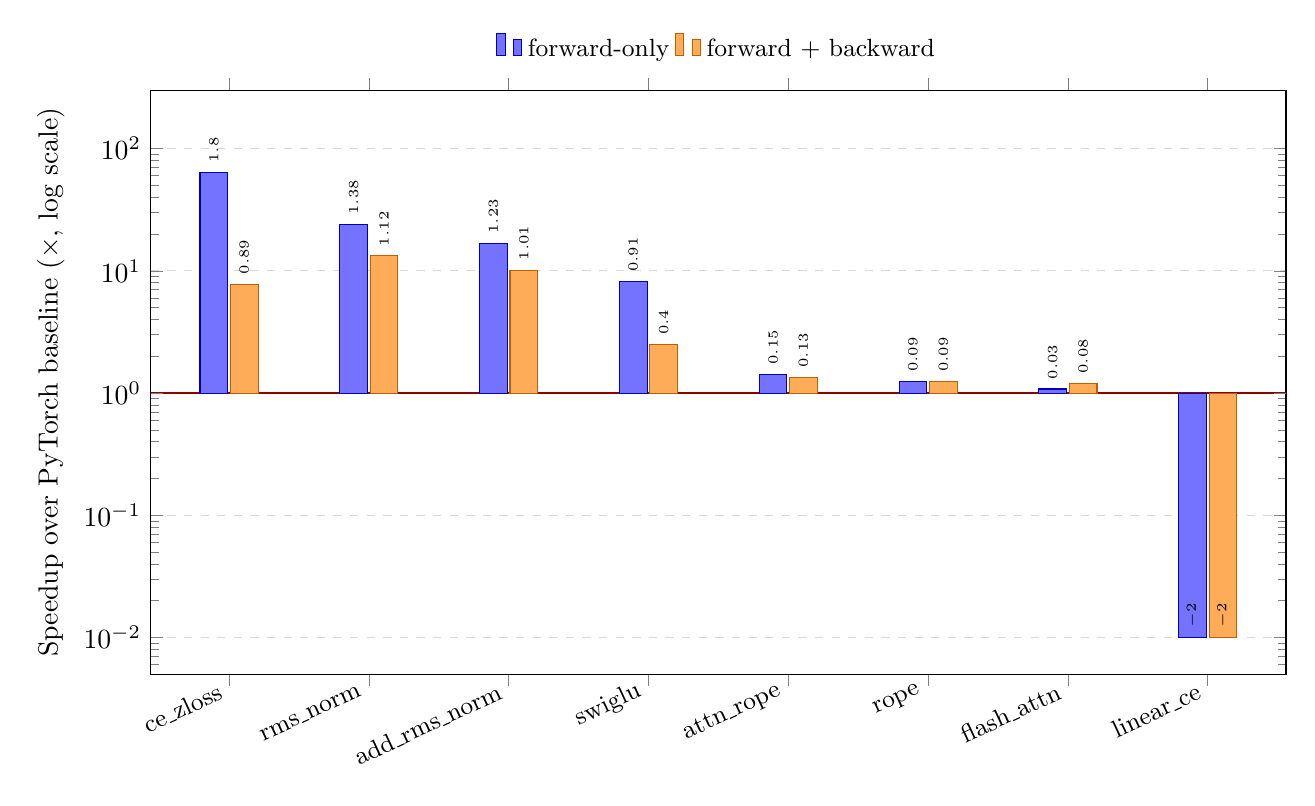
\begin{tikzpicture}
\begin{axis}[
    ybar=1pt,
    bar width=10pt,
    width=16cm,
    height=9cm,
    ymode=log,
    log basis y=10,
    ymin=0.005,
    ymax=300,
    ylabel={Speedup over PyTorch baseline ($\times$, log scale)},
    symbolic x coords={
        ce\_zloss,
        rms\_norm,
        add\_rms\_norm,
        swiglu,
        attn\_rope,
        rope,
        flash\_attn,
        linear\_ce
    },
    xtick=data,
    x tick label style={rotate=25, anchor=east, font=\small},
    enlarge x limits=0.08,
    legend style={
        at={(0.5,1.03)},
        anchor=south,
        legend columns=2,
        font=\small,
        draw=none
    },
    ymajorgrids=true,
    grid style={dashed, gray!30},
    extra y ticks={1},
    extra y tick labels={},
    extra y tick style={
        grid=major,
        grid style={solid, red!55!black, line width=0.6pt}
    },
    nodes near coords,
    every node near coord/.append style={
        font=\tiny,
        rotate=90,
        anchor=west,
        /pgf/number format/.cd, fixed, precision=2
    },
]

% forward-only speedup (蓝色) — 数据来自 profile_v2_h800.md
\addplot[fill=blue!55, draw=blue!70!black] coordinates {
    (ce\_zloss,       63.75)
    (rms\_norm,       24.00)
    (add\_rms\_norm,  16.82)
    (swiglu,           8.15)
    (attn\_rope,       1.42)
    (rope,             1.24)
    (flash\_attn,      1.08)
    (linear\_ce,       0.01)
};
\addlegendentry{forward-only}

% forward + backward speedup (橙色) — 数据来自 profile_bwd_h800.md
\addplot[fill=orange!65, draw=orange!75!black] coordinates {
    (ce\_zloss,        7.79)
    (rms\_norm,       13.26)
    (add\_rms\_norm,  10.13)
    (swiglu,           2.49)
    (attn\_rope,       1.34)
    (rope,             1.24)
    (flash\_attn,      1.20)
    (linear\_ce,       0.01)
};
\addlegendentry{forward + backward}

% baseline 1x 红色实线 (extra y tick + grid style 自动生成, 无需 \draw)

\end{axis}
\end{tikzpicture}
\end{document}

%
% 数据来源:
%   profile_v2_h800.md   (forward-only)
%   profile_bwd_h800.md  (forward + backward)
% 测试硬件: NVIDIA H800 PCIe
% 测试形状: B=64, T=3072, d_model=448, d_ff=1216, h=7, V=256, bf16
%
% 设计要点:
%   - y 轴 log scale: 数据从 0.01x (linear_ce) 到 63.75x (ce_zloss) 跨 4 个数量级
%   - x 轴按 forward-only 加速比降序排列, 视觉趋势从高到低 + 反面案例垫底
%   - 柱顶数据标签竖排, 双工作负载分组对照
\documentclass[tikz,border=10pt]{standalone}
\usepackage{pgfplots}
\usepackage{amsmath}
\pgfplotsset{compat=1.18}

\begin{document}
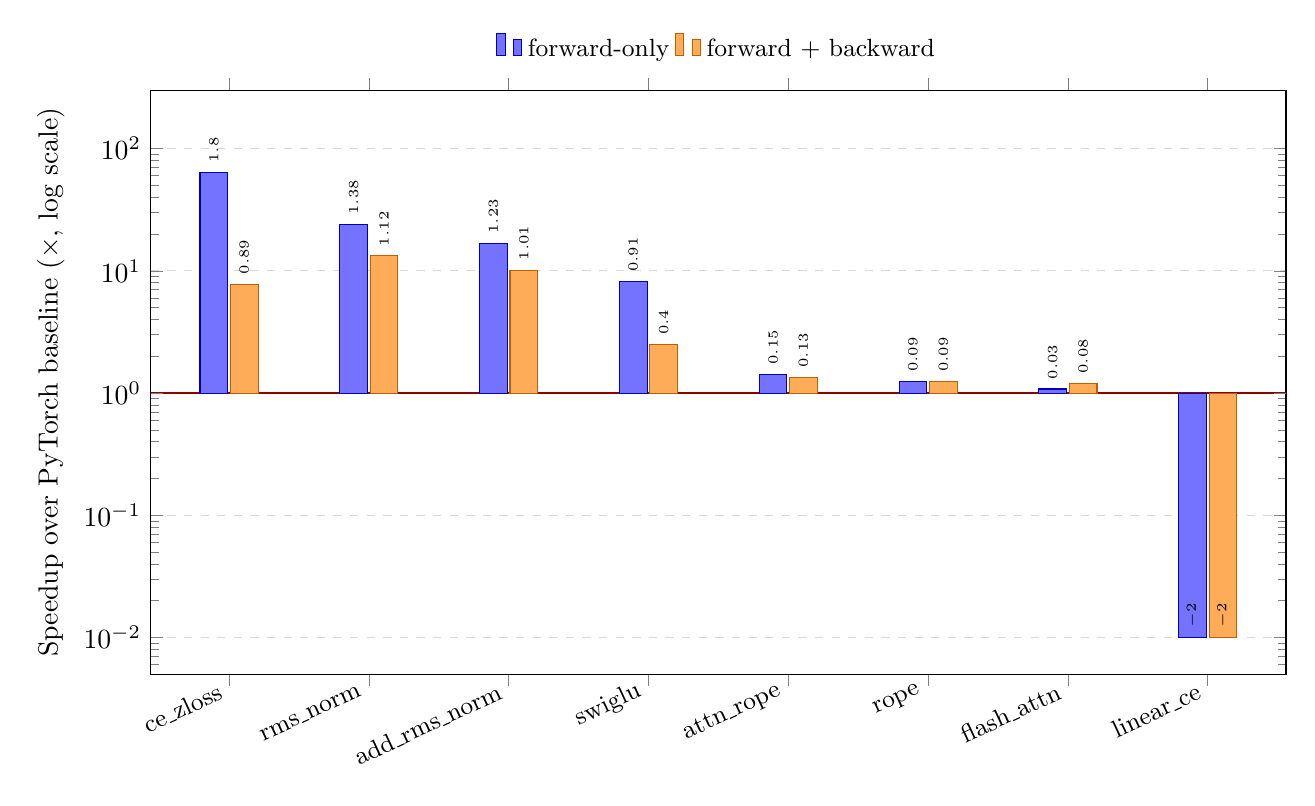
\begin{tikzpicture}
\begin{axis}[
    ybar=1pt,
    bar width=10pt,
    width=16cm,
    height=9cm,
    ymode=log,
    log basis y=10,
    ymin=0.005,
    ymax=300,
    ylabel={Speedup over PyTorch baseline ($\times$, log scale)},
    symbolic x coords={
        ce\_zloss,
        rms\_norm,
        add\_rms\_norm,
        swiglu,
        attn\_rope,
        rope,
        flash\_attn,
        linear\_ce
    },
    xtick=data,
    x tick label style={rotate=25, anchor=east, font=\small},
    enlarge x limits=0.08,
    legend style={
        at={(0.5,1.03)},
        anchor=south,
        legend columns=2,
        font=\small,
        draw=none
    },
    ymajorgrids=true,
    grid style={dashed, gray!30},
    extra y ticks={1},
    extra y tick labels={},
    extra y tick style={
        grid=major,
        grid style={solid, red!55!black, line width=0.6pt}
    },
    nodes near coords,
    every node near coord/.append style={
        font=\tiny,
        rotate=90,
        anchor=west,
        /pgf/number format/.cd, fixed, precision=2
    },
]

% forward-only speedup (蓝色) — 数据来自 profile_v2_h800.md
\addplot[fill=blue!55, draw=blue!70!black] coordinates {
    (ce\_zloss,       63.75)
    (rms\_norm,       24.00)
    (add\_rms\_norm,  16.82)
    (swiglu,           8.15)
    (attn\_rope,       1.42)
    (rope,             1.24)
    (flash\_attn,      1.08)
    (linear\_ce,       0.01)
};
\addlegendentry{forward-only}

% forward + backward speedup (橙色) — 数据来自 profile_bwd_h800.md
\addplot[fill=orange!65, draw=orange!75!black] coordinates {
    (ce\_zloss,        7.79)
    (rms\_norm,       13.26)
    (add\_rms\_norm,  10.13)
    (swiglu,           2.49)
    (attn\_rope,       1.34)
    (rope,             1.24)
    (flash\_attn,      1.20)
    (linear\_ce,       0.01)
};
\addlegendentry{forward + backward}

% baseline 1x 红色实线 (extra y tick + grid style 自动生成, 无需 \draw)

\end{axis}
\end{tikzpicture}
\end{document}

%
% 数据来源:
%   profile_v2_h800.md   (forward-only)
%   profile_bwd_h800.md  (forward + backward)
% 测试硬件: NVIDIA H800 PCIe
% 测试形状: B=64, T=3072, d_model=448, d_ff=1216, h=7, V=256, bf16
%
% 设计要点:
%   - y 轴 log scale: 数据从 0.01x (linear_ce) 到 63.75x (ce_zloss) 跨 4 个数量级
%   - x 轴按 forward-only 加速比降序排列, 视觉趋势从高到低 + 反面案例垫底
%   - 柱顶数据标签竖排, 双工作负载分组对照
\documentclass[tikz,border=10pt]{standalone}
\usepackage{pgfplots}
\usepackage{amsmath}
\pgfplotsset{compat=1.18}

\begin{document}
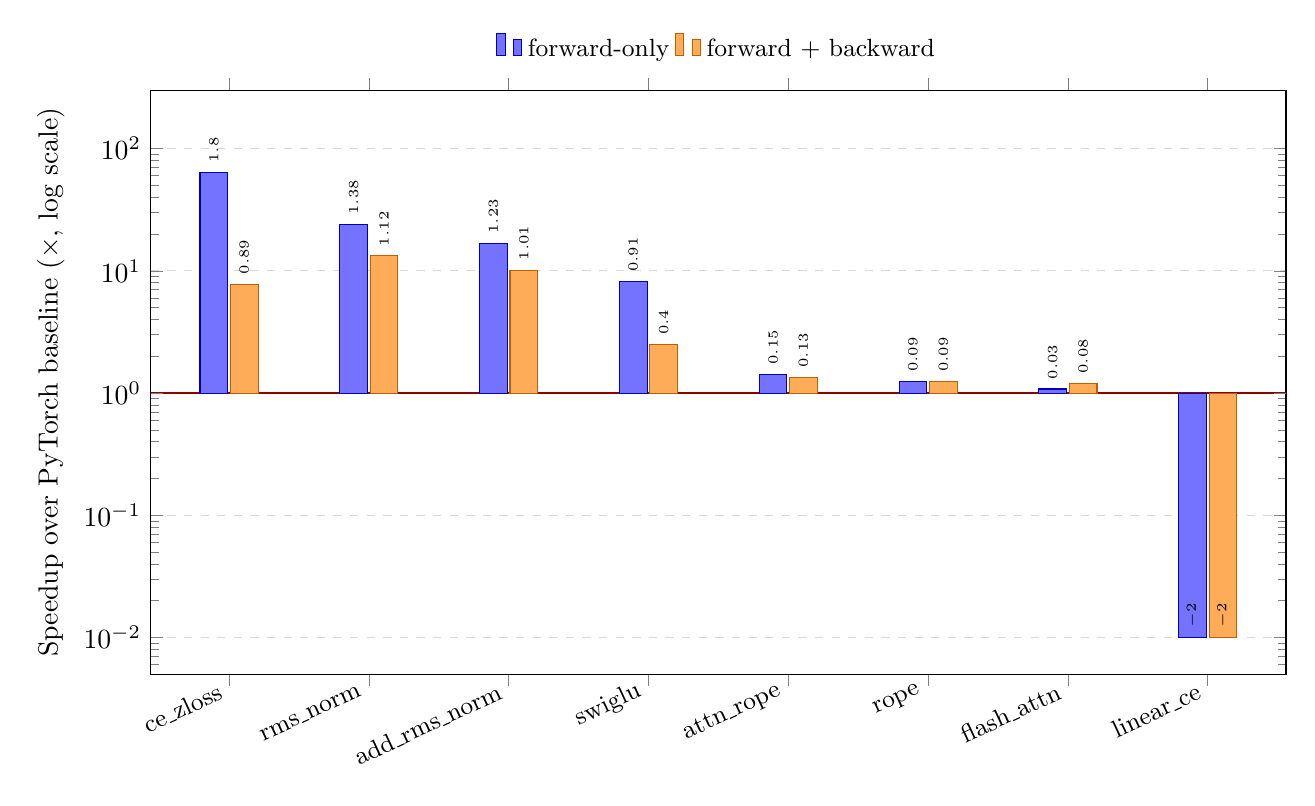
\begin{tikzpicture}
\begin{axis}[
    ybar=1pt,
    bar width=10pt,
    width=16cm,
    height=9cm,
    ymode=log,
    log basis y=10,
    ymin=0.005,
    ymax=300,
    ylabel={Speedup over PyTorch baseline ($\times$, log scale)},
    symbolic x coords={
        ce\_zloss,
        rms\_norm,
        add\_rms\_norm,
        swiglu,
        attn\_rope,
        rope,
        flash\_attn,
        linear\_ce
    },
    xtick=data,
    x tick label style={rotate=25, anchor=east, font=\small},
    enlarge x limits=0.08,
    legend style={
        at={(0.5,1.03)},
        anchor=south,
        legend columns=2,
        font=\small,
        draw=none
    },
    ymajorgrids=true,
    grid style={dashed, gray!30},
    extra y ticks={1},
    extra y tick labels={},
    extra y tick style={
        grid=major,
        grid style={solid, red!55!black, line width=0.6pt}
    },
    nodes near coords,
    every node near coord/.append style={
        font=\tiny,
        rotate=90,
        anchor=west,
        /pgf/number format/.cd, fixed, precision=2
    },
]

% forward-only speedup (蓝色) — 数据来自 profile_v2_h800.md
\addplot[fill=blue!55, draw=blue!70!black] coordinates {
    (ce\_zloss,       63.75)
    (rms\_norm,       24.00)
    (add\_rms\_norm,  16.82)
    (swiglu,           8.15)
    (attn\_rope,       1.42)
    (rope,             1.24)
    (flash\_attn,      1.08)
    (linear\_ce,       0.01)
};
\addlegendentry{forward-only}

% forward + backward speedup (橙色) — 数据来自 profile_bwd_h800.md
\addplot[fill=orange!65, draw=orange!75!black] coordinates {
    (ce\_zloss,        7.79)
    (rms\_norm,       13.26)
    (add\_rms\_norm,  10.13)
    (swiglu,           2.49)
    (attn\_rope,       1.34)
    (rope,             1.24)
    (flash\_attn,      1.20)
    (linear\_ce,       0.01)
};
\addlegendentry{forward + backward}

% baseline 1x 红色实线 (extra y tick + grid style 自动生成, 无需 \draw)

\end{axis}
\end{tikzpicture}
\end{document}
